\chapter{Návrh projektu}

\section{Výběr technologií}

\subsection{Frontend}
Trendy v oblasti vývoje webových aplikací se mění rychle avšak velkou změnou,
která ovlivnila celý způsob principu jak na stránku nahlížet přinesla technologie
\textbf{Single page aplication}, jež je implementovaná
např. v knihovně \textbf{React} zaštiťovanou společností Facebook.

\subsubsection{Single page aplication}
Single page aplication je technologie umožnující vykreslení jiné stránky,
bez nutnosti posílaní requestu na server.
Uživatel si při prvním spuštěni webu stáhne celý baliček webu a 
při opětovném načtení vetšinou sahá jen do své lokální cache.
Javascriptová knihovna (v tomto případě React)
poté stránku překresluje při uživatelské interakci.
V případě nutnosti staženi / posílaní dat mezi serverem a uživatelem
(např. editace záznamu, nebo načtení existujícího záznamu)
se volá pouze request k API webové služby a tělo requestu obsahuje pouze
užitečné (ne-redundantní) informace. 


\subsubsection{React}
Knihovna React poskytuje single page aplication technologii.
Jedná se o dobře udržovanou knihovnu, jež byla vyvinuta Facebookem, 
jakožto náhrada zastaralého konceptu renderovaní stránky na serveru.
Díky tomu servery nemusejí ztrácet výkon s každou změnou na stránce a
výkon k renderovaní se bere z PC uživatele.
Jádro této knihovny je velmi dobře optimalizované a poskytuje i řadu
debutováních nástrojů, což je pro vetší projekty nepostradatelná výhoda.  


\subsubsection{Dalsi mozne technologie}
Velmi často vykreslovaní stránek probíhá na serveru, se systémy jako jsou 
WordPress, psaný v PHP. Takovýto system je velmi dobře uživatelsky přivětivý,
ale z pohledu výkonu má velmi obrovský overhead. 
V případě implementace knihovního systému by to znamenalo vykreslovat
celou stránku (hlavičku, tělo i zápatí) na serveru,
na druhé straně single page aplication nic nerenderuje,
pouze pošle požadované informace.


\subsection{Backend}
Mít single page aplikaci na frontendu znamená, že na backendu musí existovat API,
od kterého bude frontend čerpat data.
Navíc zde potřebujeme i systém pro statické odesílaní balíku celé webové stránky.
V rámci udržitelnosti jsem se rozhodl využit jazyk Javascript stejný jako pro frontend.
Express.js je knihovna která umožňuje komplexní správu requestu a
stala se tudíž jasnou volbou.

\subsubsection{Express.js}
Express.js poskytuje odesílaní statických stránek (Reactího balíku v našem případe),
custom requesty pro rozmanité API a také odesílaní a lokální ukládaní statických souborů,
jako obrázků, wordovských i pdf dokumentů atd.

\subsubsection{MongoDB}
MongoDB je databázový system typu non-sql.
Což primárně znamená, že data neuchovává v tabulkách, ale v tkz. schématech.
Což má mnoho výhod, největší je, že nekompletní záznamy nezabírají
svými nevyplněnými daty místo v DB a ukládá se opravdu jen to co je potřeba.
Další výhodou, je styl ukládaní dat a komunikace s DB.
Databáze si data uchovává ve formátu BSON (binární JSON rozšířený o datové typy).
O data si aplikace žádá pomoci query,
která je zcela odlišná od těch u sql-like databází,
primárně se zde neposílá query ve formátu string ale jako JSON objekt,
díky čemuž např. nenastane známa SQL injection.
Znovu ve formátu JSON poté data vrací aplikaci.

\subsubsection{Další možné technologie}
Díky odděleni frontendu a backendu (narozdíl od např. WordPressu) je možné
na backend nasadit téměř cokoliv co umi posílat requesty.
Příkladem tomu můžou byt scripty v jazycích PHP, C\#, Python, nebo Perl.
Ale vzhledem k tomu, že jedním z modulů bude neuronová síť na pokročilé vyhledávaní,
vybíral jsem mezi Pythonem a JavaScriptem, jakožto 2mi jazyky, které
mají velmi dobré knihovny pro práci s neuronovými sítěmi.

\section{Diagram systému}
\noindent
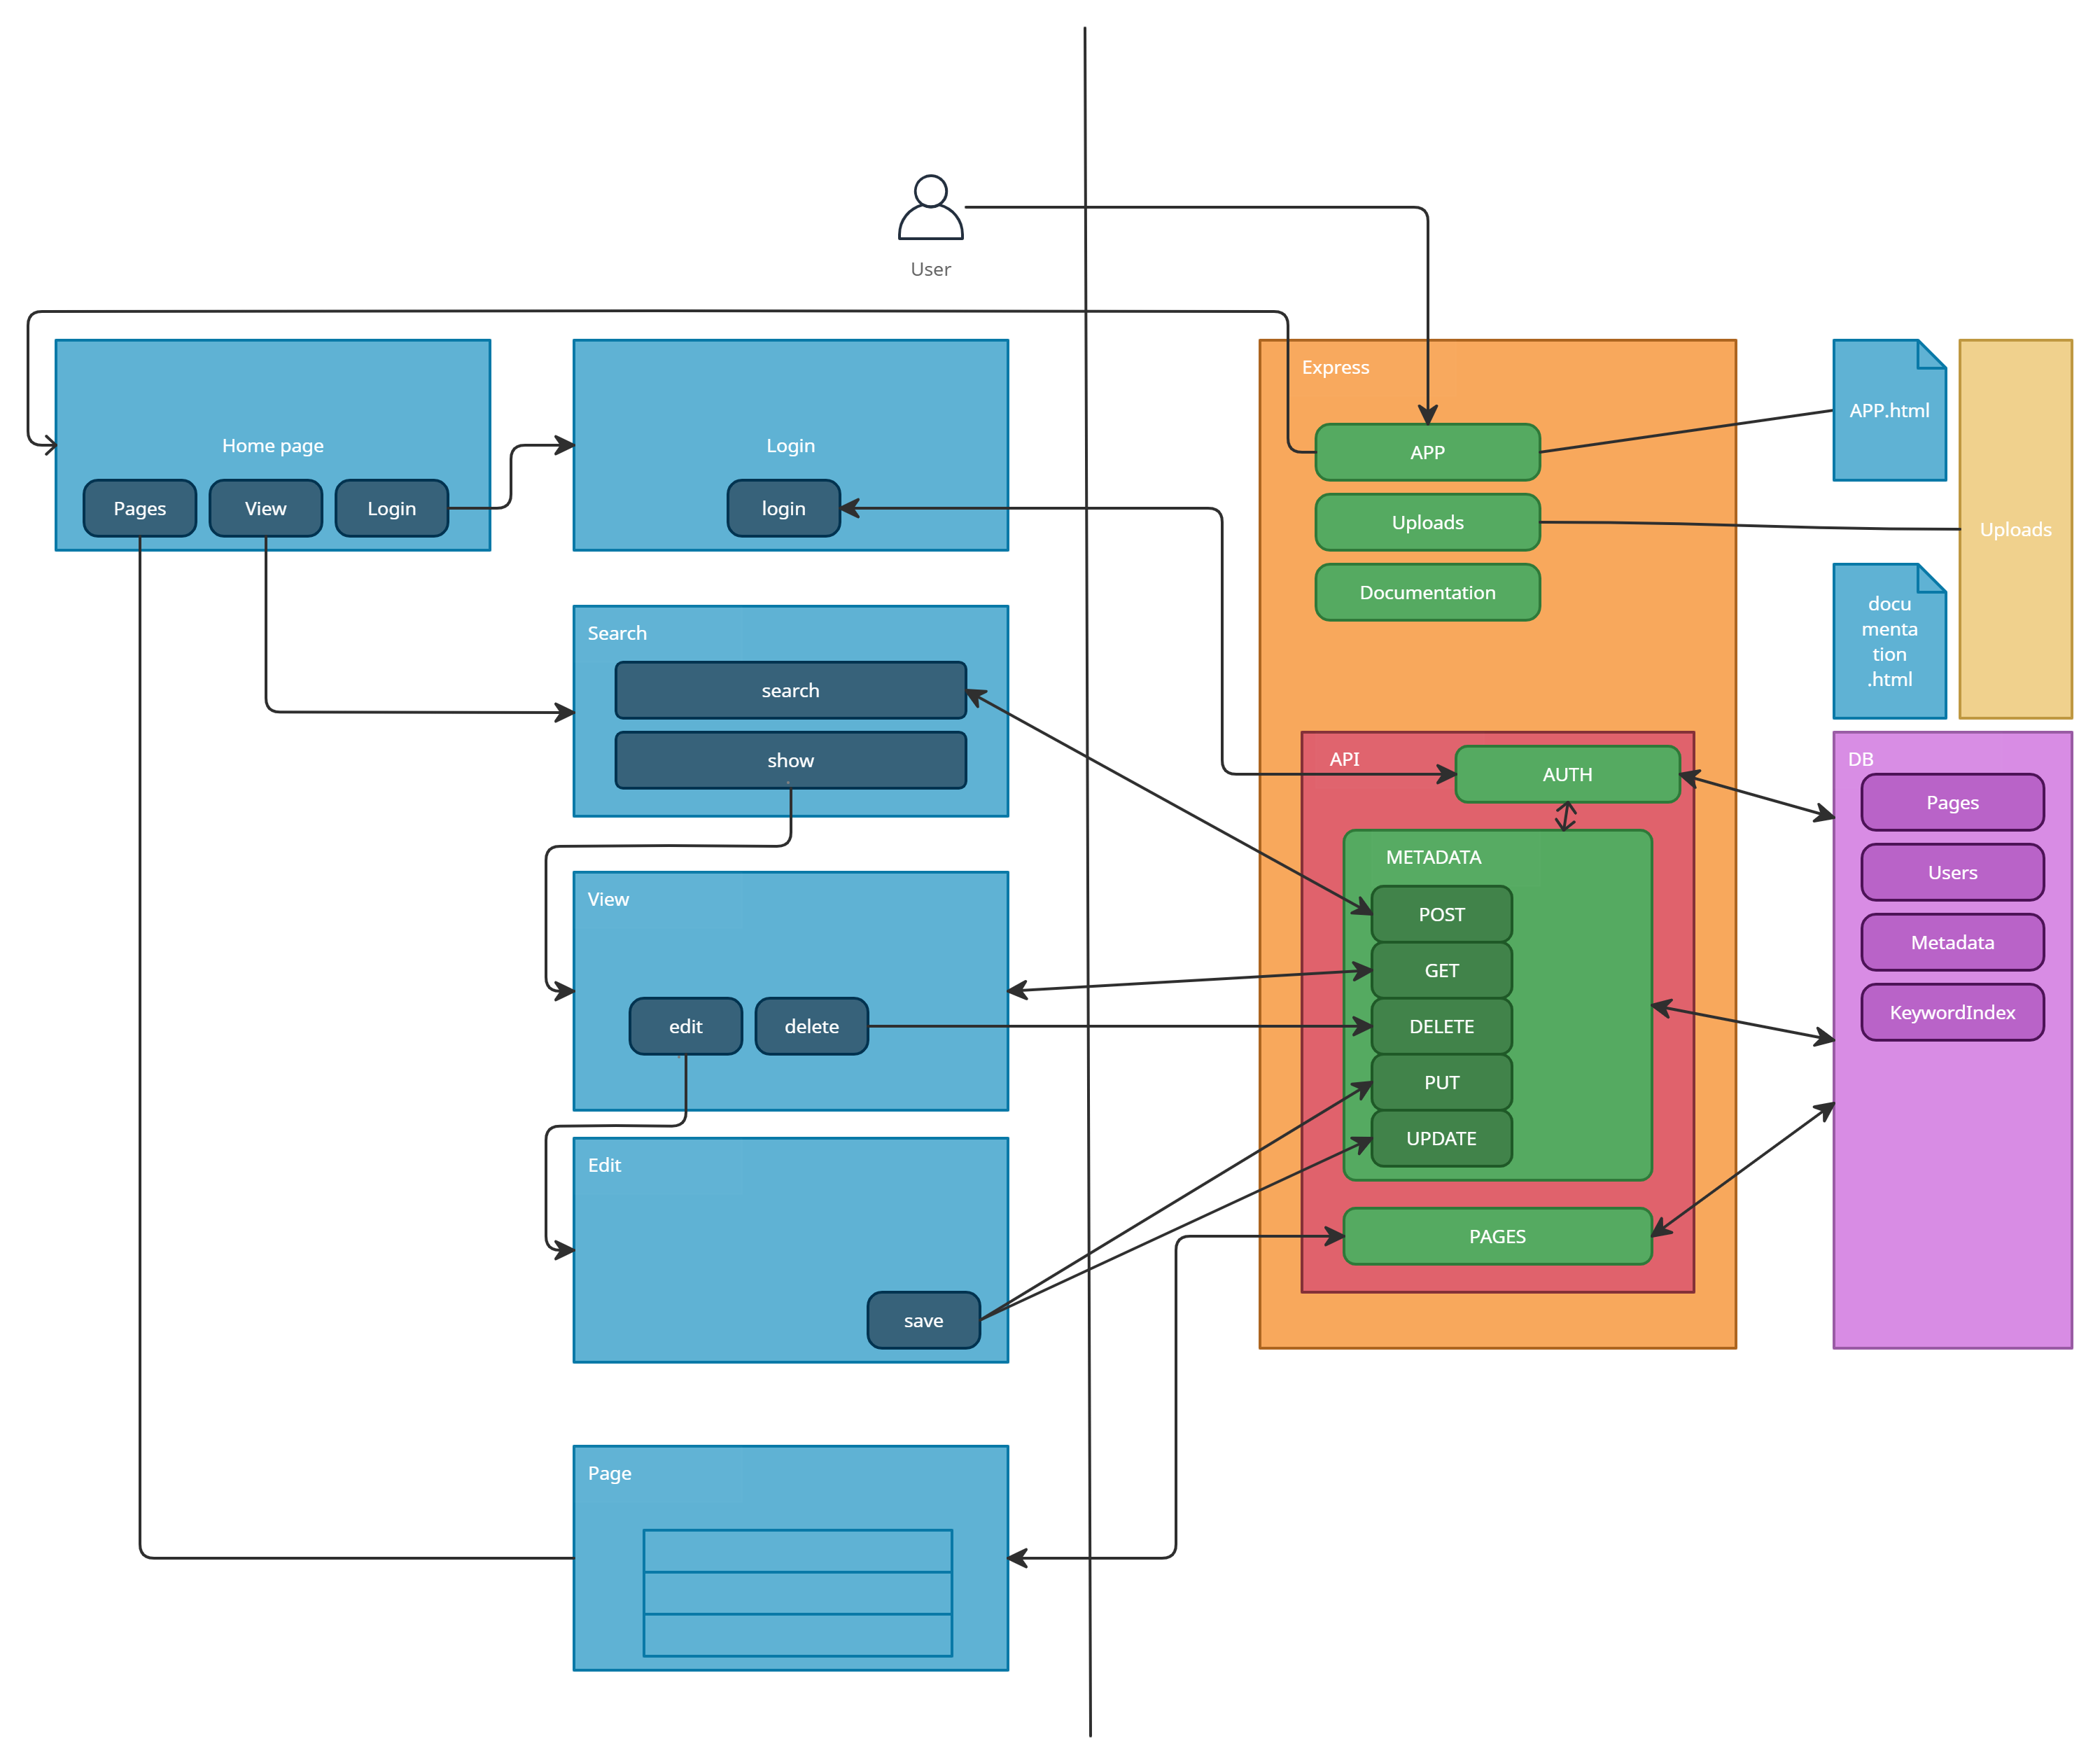
\includegraphics[angle=-90,origin=c,width=\linewidth]{img/diagram.png}
